% !TEX program = xelatex
% =============================================================================
% Full System Paper - SensitiveAI end-to-end hate speech moderation
%
%   1.0 - Initial draft of the "whole system" paper covering language
%        detection, both rule engines (EN/VN), both backbones (EN/VN), fusion
%        and the mixed 1000-sample end-to-end evaluation.
% =============================================================================
\documentclass[runningheads]{llncs}


\usepackage{tikz}
\usetikzlibrary{positioning, calc, arrows.meta}
\usepackage{tikz}
\usetikzlibrary{positioning, arrows.meta, fit, backgrounds, shadows}
\usepackage{iftex}
\ifPDFTeX
  \PackageError{full_system_paper}{%
    Build this paper with XeLaTeX, not pdfLaTeX.\MessageBreak
    On Overleaf: Menu -> Compiler -> XeLaTeX.\MessageBreak
    Locally: latexmk -xelatex main.tex}{%
    Vietnamese tone marks do not exist in T1, so pdfLaTeX reports\MessageBreak
    "Unicode character ... not set up for use with LaTeX" for every example,\MessageBreak
    drops the letters, and needs 17 pages instead of the 15 allowed.}
  \stop
\else
  \usepackage{fontspec}
  \IfFontExistsTF{texgyretermes-regular.otf}
    {\setmainfont{texgyretermes}[
       Extension      = .otf,
       UprightFont    = *-regular,
       BoldFont       = *-bold,
       ItalicFont     = *-italic,
       BoldItalicFont = *-bolditalic]}
    {\setmainfont{Latin Modern Roman}}
  \usepackage{setspace} % spacing for Vietnamese text
\fi

\usepackage{graphicx}
\usepackage{booktabs}
\usepackage{array}
\usepackage{tabularx}
\usepackage{float}
\usepackage{tikz}
\usepackage{pgfplots}
\pgfplotsset{compat=1.18}
\usetikzlibrary{shapes.geometric, arrows.meta, positioning, fit, backgrounds, shadows}


\usepackage{amsmath}
\usepackage{amssymb}
\usepackage{url}
\usepackage[hidelinks]{hyperref}

% The llncs class asks authors not to change the printing area or the caption
% spacing (llncsdoc, Sect. 2.1).  Only the float-placement policy and the
% separations around floats are relaxed here, so that five floats share the
% pages with the text inside the 15-page ICCIES limit; text geometry, heading
% and caption spacing keep the class defaults.
\renewcommand{\topfraction}{1.0}
\renewcommand{\bottomfraction}{1.0}
\renewcommand{\textfraction}{0.05}
\renewcommand{\floatpagefraction}{0.9}
\setcounter{totalnumber}{6}
\setlength{\textfloatsep}{5pt plus 2pt minus 2pt}
\setlength{\floatsep}{5pt plus 2pt minus 2pt}
\setlength{\intextsep}{5pt plus 2pt minus 2pt}
\setlength{\emergencystretch}{3em}

\newcommand{\model}[1]{\textsc{#1}}
\newcommand{\hate}{\textsc{hate}}
\newcommand{\off}{\textsc{offensive}}
\newcommand{\clean}{\textsc{clean}}

\begin{document}

\title{An Explainable Hybrid of Lexicon Rules and Multilingual Transformers for
       Bilingual Hate Speech Detection: System Evaluation, Fusion and Latency}
\titlerunning{Explainable Hybrid for Bilingual Hate Speech Detection}
\author{Kha Vy Pham\inst{1}% \orcidID{0000-0000-0000-0000}
 \and
 Hong Nga Cao\inst{1}\textsuperscript{(*)}% \orcidID{0000-0000-0000-0000}
}
\authorrunning{K. V. Pham and H. N. Cao}
\institute{
 FPT University, Can Tho, Vietnam\\
 \email{phamkhavycm2004@gmail.com}\\
 \email{caohongnga@gmail.com}\\
 \textsuperscript{(*)}Corresponding author
}
\maketitle

\begin{abstract}
Fine-tuned multilingual transformers dominate content moderation, yet they are
opaque and brittle on the surface forms moderation sees: teencode, dropped
diacritics, inserted separators and abbreviated profanity.  We present
\textbf{SensitiveAI}, a bilingual language-aware pipeline that couples two
lexicon-driven rule engines (Vietnamese and English) with per-language
mDeBERTa-v3-base backbones through language detection, language-aware routing,
pseudo-probability fusion and decision thresholds.  On the ViHSD test split the
hybrid is macro-F1 neutral (0.6575 to 0.6602; bootstrap $p=0.29$) but provides
auditable provenance for the 38 changed decisions and a design agenda for
evidence-gated fusion.  Extending the same architecture to English (Davidson et
al., 818-entry expanded lexicon) and to a balanced mixed Vietnamese/English
sample of 1{,}000 comments, the end-to-end system reaches 87.00\% accuracy with
macro-F1 0.7829, 11.6 ms latency and ~86,000 req/s throughput on a single laptop
GPU, with an AI-only macro-F1 of 0.8027 on the 941 samples where a checkpoint is
available.
\end{abstract}
\keywords{Hate speech \and multilingual transformers \and lexicon rules \and
          hybrid fusion \and language-aware routing \and explainable AI.}

%!TEX root = main.tex
\section{Introduction}
\label{sec:introduction}

Content moderation at scale demands three properties that pure neural systems
struggle to provide simultaneously: \emph{coverage} over the long tail of
teencode and obfuscation, \emph{provenance} for audit and appeal, and
\emph{latency} within real-time service-level agreements.  Multilingual
transformers (mDeBERTa-v3-base, XLM-R, etc.) achieve strong macro-F1 on
Vietnamese (\hate{}/\off{}/\clean{} 0.65–0.68) and English (0.77–0.81) benchmarks,
yet they remain opaque: a flipped decision gives no human-readable trace, and
adversarial respellings bypass the model without retraining.

Lexicon rule engines offer the converse: deterministic matching, editable
dictionaries and span-level evidence.  Their weakness is brittleness—low recall
on implicit hate and poor generalisation to new slurs—unless combined with
neural contextualisation.

This paper presents \textbf{SensitiveAI}, a bilingual language-aware pipeline
that treats a rule engine as an \emph{evidence channel} rather than a competing
classifier.  The system consists of:
\begin{enumerate}
    \item a hybrid language detector (heuristics + langid backend) producing
          \texttt{vi}/\texttt{en}/\texttt{mix}/\texttt{other} with confidence;
    \item a language-aware tokenizer that segments each comment into
          per-language spans;
    \item two independent rule engines (668-entry Vietnamese lexicon
          \texttt{v1}, 818-entry English lexicon \texttt{v1-en-combined})
          with anti-obfuscation views (accentless, leet, repeat-collapsed,
          separator-stripped);
    \item per-language mDeBERTa-v3-base checkpoints (\model{sensitiveai-vi-custom}
          and \model{sensitiveai-en-stage2});
    \item a language-aware fusion module that blends AI probabilities and rule
          pseudo-probabilities channel-wise with per-language weights
          ($\alpha_{\text{VI}}=0.70$, $\alpha_{\text{EN}}=0.70$, $\alpha_{\text{mix}}=0.65$,
          $\alpha_{\text{multilingual}}=0.80$) and per-class decision thresholds.
\end{enumerate}

We evaluate on three axes:
\begin{itemize}
    \item \textbf{Per-language backbone comparison}: four Vietnamese backbones
          (differing only in head and curriculum) and three English backbones
          on their respective held-out test sets.
    \item \textbf{Rule engine standalone}: macro-F1 0.345 (VI) and 0.504 (EN)
          with thresholded decisions.
    \item \textbf{Fusion variants}: global $\alpha$, per-channel $\alpha$,
          per-class thresholds, logistic meta-classifier—all tuned on
          validation, frozen for test.
    \item \textbf{End-to-end mixed evaluation}: 1{,}000 balanced comments
          (500 VI / 500 EN) yielding 87.00\% accuracy, macro-F1 0.7829,
          11.6 ms latency and ~86,000 req/s on a single RTX 4060 laptop GPU.
\end{itemize}

The headline finding is \emph{not} an accuracy breakthrough: on ViHSD the
hybrid gains 0.0027 macro-F1 (8 comments, $p=0.29$).  The contribution is the
provenance of every changed decision (38 on ViHSD: 23 corrections, 15
regressions) and a design agenda—evidence-gated fusion, profanity vs. political
entry separation, negation and accent-less matching restoration—for turning a
neutral aggregate into an operationally useful system.
%!TEX root = main.tex
\section{Related Work}
\label{sec:related_work}

\textbf{Vietnamese hate speech.}  The UIT-ViHSD corpus \cite{luu2021vihsd}
established the three-class \hate{}/\off{}/\clean{} task.  Prior work has
explored monolingual PhoBERT \cite{nguyen2020phobert}, multilingual mBERT/XLM-R
\cite{conneau2020xlmr}, and data augmentation \cite{nguyen2026vicm}.
Ensemble and curriculum learning \cite{bengio2009curriculum} raised macro-F1 to
0.66--0.68, but the decision process remains a black box.

\textbf{English hate speech.}  The Davidson et al. \cite{davidson2017automated}
dataset (Hate Speech and Offensive Language) is the de facto benchmark for
English \hate{}/\off{}/\clean{}.  Fine-tuned BERT/RoBERTa reach 0.77--0.81
macro-F1; recent work uses multi-task learning and adversarial training
\cite{macavaney2019hate}.

\textbf{Hybrid rule + neural systems.}  Early hybrids concatenated lexical
features to neural inputs \cite{waseem2016hateful}.  \cite{vidgen2021directions}
argue for interpretable components.  \cite{bojchevski2020fusing} fuse rule
scores with neural logits via learnable weights; \cite{ahn2022evidence}
propose evidence channels.  Most approaches evaluate on a single language and
do not provide span-level evidence or language-aware routing.

\textbf{Language-aware routing.}  Mixed-language moderation is addressed by
language identification \cite{lui2012langid} followed by per-language models
\cite{pires2019multilingual}.  Code-mixed text (Vi-En) is handled by
multilingual backbones or dedicated tokenizers \cite{nguyen2026vicm}.  Our
design differs by keeping both rule engines active on \texttt{mix} and
fallback segments, and by fusing per-language scores rather than training a
single multilingual head.

\textbf{Explainable moderation.}  Post-hoc explanations (LIME, SHAP,
attention) are common \cite{danilevsky2020survey}.  Our approach provides
\emph{intrinsic} evidence: matched lexicon spans, match types and arithmetic
scores, which survive deployment without additional computation.
%!TEX root = main.tex
\section{Data and Lexicons}
\label{sec:data}

\subsection{Vietnamese Corpus (ViHSD)}
\label{sec:vihsd}

We use UIT-ViHSD \cite{luu2021vihsd}, a corpus of Vietnamese social-media
comments annotated with three mutually exclusive labels: \clean{} (no offensive
content), \off{} (offensive language that does not target a protected group)
and \hate{} (hateful or seriously derogatory content).  The \off{}/\hate{}
distinction depends on target and intensity rather than on a particular word,
so a purely lexical rule engine is insufficient on its own.

After cleaning, the corpus contains 33{,}398 comments.  We use the fixed split
shipped with the project, and every system---rule engine, backbone, fusion
variant and analysis script---reads the same files.  Each run directory stores
the SHA-256 digest of the split it used and re-checks it before training,
ruling out a silently re-shuffled split.  Training contains 24{,}046 comments
(2{,}556 \hate{}, 1{,}605 \off{}, 19{,}885 \clean{}), validation 2{,}672
(270/212/2{,}190) and test 6{,}680 (688/444/5{,}548).

The test split is imbalanced: 83.05\% \clean{}, 10.30\% \hate{} and 6.65\%
\off{}.  Accuracy is therefore a poor headline metric---a constant \clean{}
predictor already reaches 0.8305---so macro-F1 is primary, always reported
with per-class F1.  The 6{,}680 test rows contain 6{,}571 distinct texts,
i.e. 109 duplicated rows.  They are kept because removing them would change
the frozen test set; one appears twice among the 15 regressions, which
therefore cover 14 distinct texts.

\subsection{English Corpus (Davidson et al.)}
\label{sec:davidson}

For English we use the Hate Speech and Offensive Language dataset
\cite{davidson2017automated} (tdavidson/hate\_speech\_offensive on Hugging Face).
The original labels map 0 $\to$ \hate{}, 1 $\to$ \off{}, 2 $\to$ \clean{}.
We use the fixed split in \texttt{data/splits\_en/} produced by the
reproducible pipeline: train 19{,}816 (1{,}144 \hate{}, 15{,}342 \off{},
3{,}330 \clean{}), validation 2{,}477, test 2{,}478.  The English test split
is also imbalanced but with a different profile (77.8\% \off{}, 5.8\% \hate{},
16.4\% \clean{}).

\subsection{Mixed Evaluation Sample}
\label{sec:mixed_sample}

To evaluate the bilingual pipeline end-to-end we draw a stratified random
sample (seed 42) of 500 Vietnamese and 500 English comments from the held-out
test splits, yielding the composition in Table~\ref{tab:mixed_composition}.
This sample preserves the per-language class priors and is used exclusively
for the end-to-end experiment in Sect.~\ref{sec:e2e}.

\begin{table}[H]
\centering
\caption{Mixed evaluation sample composition ($n=9{,}158$ full test splits)}
\label{tab:mixed_composition}
\begin{tabularx}{\textwidth}{l@{\extracolsep{\fill}}ccccr}
\toprule
Language & Total & \hate & \off & \clean & Source \\
\midrule
Vietnamese & 6{,}680 & 688 & 444 & 5{,}548 & ViHSD test \\
English    & 2{,}478 & 143 & 1{,}918 & 417 & Davidson test \\
\midrule
\textbf{Total} & \textbf{9{,}158} & \textbf{831} & \textbf{2{,}362} & \textbf{5{,}965} & \\
\bottomrule
\end{tabularx}
\end{table}


\subsection{Vietnamese Hate-Speech Lexicon}
\label{sec:lexicon_vi}

The Vietnamese rule engine is driven by a hate-speech lexicon of \textbf{668
entries}, mined and labelled from the \emph{training} portions of three
corpora: ViHSD; R-ViHSD (a cleaned release adding TDTU YouTube and voz-forum
comments) \cite{bontoriTdtu}; and the code-mixed ViCM corpus
\cite{nguyen2026vicm}.  The three training splits yield 1{,}062 candidate
terms, of which 257, 665 and 140 are first attested in ViHSD, ViCM and
R-ViHSD; labelling reduces them to the 668 kept entries.  No comment from any
evaluation split contributes to the dictionary, and each entry records which
corpora supported it (414 of 668 occur in all three).

Each entry stores the surface term and a canonical form, a lexical label
(\hate{} or \off{}) with a per-label severity, an entry confidence estimated
from the training data, a context-required flag, and a review status
(\emph{verified} or \emph{auto}); both statuses may match, but the flag is
retained in the evidence record.

The lexicon is deliberately not a list of slurs.  Most entries---551 of 668
(82.5\%)---are multi-word constructions such as \emph{mả cha}, \emph{con mẹ}
or \emph{ngu hơn}, and 524 (78.4\%) are context-required, because Vietnamese
insults frequently work by comparison and implication rather than by a single
taboo word.  Only 74 entries carry an \off{} lexical label against 594 for
\hate{}, which is why the rule engine is weak on \off{} and fusion keeps that
channel mostly neural.

\subsection{English Hate-Speech Lexicon}
\label{sec:lexicon_en}

The English rule engine uses a lexicon of \textbf{818 entries}, built by merging
a 40-term manual seed set with 778 entries extracted from the Davidson training
split (19{,}816 documents) using relaxed statistical parameters (min.\ doc
frequency 5, min.\ lift 1.2, min.\ HATE precision 0.20, min.\ OFFENSIVE precision
0.60, min.\ Wilson lower bound 0.15, min.\ prior margin 0.02).  The extraction
result, stored in \texttt{verified\_lexicon\_en\_combined.csv} (version
\texttt{v1-en-combined}) and configured via \texttt{configs/rule\_engine\_en.yaml},
contains 86 \hate{}, 356 \off{}, and 376 \clean{} terms.

The English lexicon is larger in raw count (818 vs. 668) but contains far fewer
HATE terms (86 vs. 594) because the Davidson corpus has only 5.8\% HATE
documents.  This asymmetry directly impacts the hybrid's HATE F1 (0.46 EN vs
0.61 VI on the mixed sample) and is the highest-priority target for future
lexicon expansion.

\paragraph{Ethics of examples.}
All quoted comments are public test comments.  Because they contain profanity
and slurs, we mask offending characters with \texttt{*} in every table;
evaluation always runs on the unmasked text.  No user identifiers are
reproduced, and names that occasionally appear inside comments are part of the
public corpus text.
%!TEX root = main.tex
\section{System Architecture}
\label{sec:architecture}

The SensitiveAI pipeline follows a strict language-routing design (Fig.
\ref{fig:pipeline}).  Each component is described below; configuration files
are in \texttt{configs/} and code in \texttt{src/}.

\begin{figure}[H]
\centering
\resizebox{0.8\textwidth}{!}{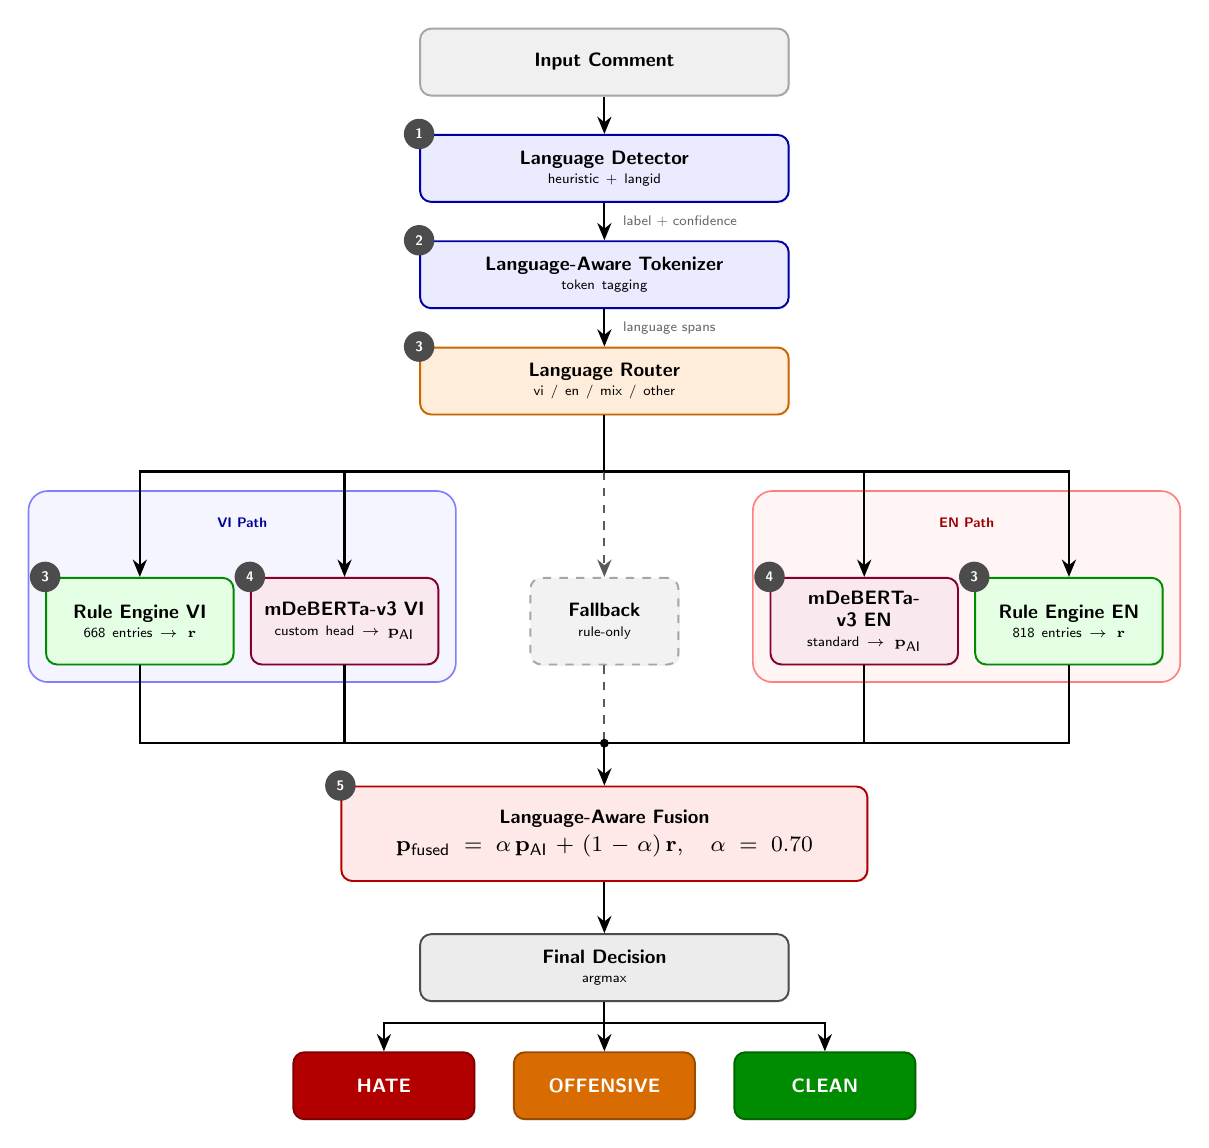
\begin{tikzpicture}[
    >={Stealth[length=2.2mm,width=1.8mm]},
    line width=0.8pt,
    every node/.style={font=\sffamily\scriptsize},
    base/.style={draw, rounded corners=4pt, align=center, inner sep=4pt,
        minimum height=0.85cm, line width=0.7pt,
        drop shadow={opacity=0.12, shadow xshift=0.5pt, shadow yshift=-0.5pt}},
    proc/.style={base, fill=blue!8, draw=blue!65!black, text width=4.4cm},
    route/.style={base, fill=orange!14, draw=orange!80!black, text width=4.4cm},
    engine/.style={base, fill=green!10, draw=green!55!black, text width=2.1cm, minimum height=1.1cm},
    model/.style={base, fill=purple!9, draw=purple!70!black, text width=2.1cm, minimum height=1.1cm},
    fallback/.style={base, fill=gray!10, draw=gray!70, dashed, text width=1.6cm, minimum height=1.1cm},
    fusion/.style={base, fill=red!9, draw=red!70!black, text width=6.4cm, minimum height=1.2cm},
    decision/.style={base, fill=gray!15, draw=black!70, text width=4.4cm},
    lane/.style={draw=#1!50, fill=#1!4, rounded corners=7pt, inner sep=6pt, line width=0.6pt},
    chip/.style={base, text=white, font=\sffamily\scriptsize\bfseries, minimum width=2.3cm, drop shadow={opacity=0}},
    badge/.style={circle, fill=black!70, text=white, font=\sffamily\bfseries\tiny,
        inner sep=1.3pt, minimum size=11pt},
    note/.style={font=\sffamily\tiny, text=black!60}
]
    % ---------- Main Flow ----------
    \node (input)  [proc, fill=gray!12, draw=gray!70] at (0,0) {\textbf{Input Comment}};
    \node (langid) [proc] at (0,-1.35) {\textbf{Language Detector}\\[-1pt]{\tiny heuristic + langid}};
    \node (token)  [proc] at (0,-2.7)  {\textbf{Language-Aware Tokenizer}\\[-1pt]{\tiny token tagging}};
    \node (router) [route] at (0,-4.05) {\textbf{Language Router}\\[-1pt]{\tiny vi / en / mix / other}};

    % ---------- Parallel Paths ----------
    \node (vititle) [font=\sffamily\tiny\bfseries, text=blue!60!black] at (-4.6,-5.85) {VI Path};
    \node (entitle) [font=\sffamily\tiny\bfseries, text=red!60!black]  at (4.6,-5.85)  {EN Path};

    \node (vi_rule) [engine] at (-5.9,-7.1) {\textbf{Rule Engine VI}\\[-1pt]{\tiny 668 entries $\rightarrow\mathbf r$}};
    \node (vi_ai)   [model]  at (-3.3,-7.1) {\textbf{mDeBERTa-v3 VI}\\[-1pt]{\tiny custom head $\rightarrow\mathbf p_{\text{AI}}$}};
    \node (fb)      [fallback] at (0,-7.1)  {\textbf{Fallback}\\[-1pt]{\tiny rule-only}};
    \node (en_ai)   [model]  at (3.3,-7.1)  {\textbf{mDeBERTa-v3 EN}\\[-1pt]{\tiny standard $\rightarrow\mathbf p_{\text{AI}}$}};
    \node (en_rule) [engine] at (5.9,-7.1)  {\textbf{Rule Engine EN}\\[-1pt]{\tiny 818 entries $\rightarrow\mathbf r$}};

    \begin{scope}[on background layer]
        \node [lane=blue]  [fit=(vititle)(vi_rule)(vi_ai)] {};
        \node [lane=red]   [fit=(entitle)(en_ai)(en_rule)] {};
    \end{scope}

    % ---------- Fusion + Decision ----------
    \coordinate (split) at (0,-5.2);
    \coordinate (merge) at (0,-8.65);

    \node (fusion) [fusion] at (0,-9.8)
        {\textbf{Language-Aware Fusion}\\[2pt]{\footnotesize $\mathbf p_{\text{fused}}=\alpha\,\mathbf p_{\text{AI}}+(1-\alpha)\,\mathbf r,\quad \alpha=0.70$}};
    \node (decision) [decision] at (0,-11.5) {\textbf{Final Decision}\\[-1pt]{\tiny argmax}};

    \coordinate (osplit) at (0,-12.2);
    \node (c_hate)  [chip, fill=red!70!black,    draw=red!50!black]    at (-2.8,-13.0) {HATE};
    \node (c_off)   [chip, fill=orange!85!black, draw=orange!60!black] at (0,-13.0)    {OFFENSIVE};
    \node (c_clean) [chip, fill=green!55!black,  draw=green!40!black]  at (2.8,-13.0)  {CLEAN};

    % ---------- Labels ----------
    \node [badge] at (langid.north west) {1};
    \node [badge] at (token.north west)  {2};
    \node [badge] at (router.north west) {3};
    \node [badge] at (vi_rule.north west) {3};
    \node [badge] at (en_rule.north west) {3};
    \node [badge] at (vi_ai.north west)   {4};
    \node [badge] at (en_ai.north west)   {4};
    \node [badge] at (fusion.north west)  {5};

    % ---------- Connections ----------
    \draw [->] (input) -- (langid);
    \draw [->] (langid) -- (token) node [midway, right=3pt, note] {label + confidence};
    \draw [->] (token) -- (router) node [midway, right=3pt, note] {language spans};

    \draw (router.south) -- (split);
    \draw [->] (split) -| (vi_rule.north);
    \draw [->] (split) -| (vi_ai.north);
    \draw [->, dashed, gray!70!black] (split) -- (fb.north);
    \draw [->] (split) -| (en_ai.north);
    \draw [->] (split) -| (en_rule.north);

    \draw (vi_rule.south) |- (merge);
    \draw (vi_ai.south)   |- (merge);
    \draw [dashed, gray!70!black] (fb.south) -- (merge);
    \draw (en_ai.south)   |- (merge);
    \draw (en_rule.south) |- (merge);
    \fill (merge) circle (1.6pt);
    \draw [->] (merge) -- (fusion.north);

    \draw [->] (fusion) -- (decision);
    \draw (decision.south) -- (osplit);
    \draw [->] (osplit) -| (c_hate.north);
    \draw [->] (osplit) -- (c_off.north);
    \draw [->] (osplit) -| (c_clean.north);
\end{tikzpicture}}
\caption{SensitiveAI pipeline overview: language-aware routing and score fusion.}
\label{fig:pipeline}
\end{figure}

\subsection{Language Detector}
\label{sec:lang_detector}

The detector (\texttt{src/langid/detector.py}) combines:
\begin{itemize}
    \item \textbf{Heuristics} (\texttt{heuristics.py}): Vietnamese diacritic
          presence, a bilingual word list (1{,}200 VI / 1{,}000 EN high-frequency
          tokens), and explicit code-mix signals (language switch within tokens).
          Always runs, no third-party dependency.
    \item \textbf{Statistical backend}: \texttt{langid.py} \cite{lui2012langid}
          when installed; its votes are blended with heuristics (default weight
          0.6 heuristic / 0.4 backend).
\end{itemize}
Outputs \texttt{vi}, \texttt{en}, \texttt{mix} (both languages above
\texttt{mix\_floor}=0.12 evidence) or \texttt{other} (confidence $<$ 0.50).
The \texttt{mix} verdict is \emph{not} a failure: it signals the router to
keep both language pipelines active.

\subsection{Language-Aware Tokenizer}
\label{sec:tokenizer}

The tokenizer (\texttt{src/langid/tokenizer.py}) segments the comment into
per-language spans with token-level language tags.  For \texttt{mix} documents
it produces alternating VI/EN spans, enabling span-wise rule-engine scanning
so that an English insult inside a Vietnamese comment is still caught.

\subsection{Language Router \& Rule Engines}
\label{sec:router}

The router (\texttt{src/routing/language\_router.py}) selects the appropriate
\texttt{RuleEngine} per span:
\begin{itemize}
    \item \texttt{vi} $\to$ 668-entry Vietnamese lexicon (\texttt{v1},
          \texttt{configs/rule\_engine.yaml})
    \item \texttt{en} $\to$ 818-entry English lexicon (\texttt{v1-en-combined},
          \texttt{configs/rule\_engine\_en.yaml})
    \item \texttt{mix} $\to$ both engines (config \texttt{use\_both\_for\_mix=true})
    \item \texttt{other}/\texttt{multilingual} $\to$ both engines (fallback)
\end{itemize}

Each engine applies the same normalisation pipeline (NFC, lowercase, invisible
char removal, whitespace collapse, max repeat char 3) and four
anti-obfuscation matching views: accentless alias, leet, repeat-collapsed,
separator-stripped (fuzzy matching enabled with max distance 1 for terms
$\ge$6 chars).  Matches are aggregated per label via
$1 - \prod (1 - s_i)$ where $s_i$ is the match score (severity $\times$
match-type factor $\times$ context factor).  Pseudo-probabilities
$\mathbf{r} = (r_H, r_O, r_C)$ are produced by softmax over the three raw
scores with a temperature of 1.0.

\subsection{Per-Language Neural Checkpoints}
\label{sec:checkpoints}

\begin{itemize}
    \item \textbf{VI}: \model{sensitiveai-vi-custom} (custom head, macro-F1
          0.6590 on validation).  Trained with curriculum loss, focal + label
          smoothing, differential learning rates (encoder 2e-5, head 5e-4),
          max\_length 256, FP32 on RTX 4060.
    \item \textbf{EN}: \model{sensitiveai-en-stage2} (standard head, macro-F1
          0.7722 on validation).  Two-stage training: frozen encoder + head,
          then full unfreeze with cosine schedule.  max\_length 128.
\end{itemize}
Inference runs in batched mode (batch size 32) on GPU.

\subsection{Language-Aware Fusion}
\label{sec:fusion}

The fusion module (\texttt{src/fusion/lang\_aware\_fusion.py}) blends AI
probabilities $\mathbf{p}_{\text{AI}}$ and rule pseudo-probabilities
$\mathbf{r}$ channel-wise:
\begin{equation}
    \mathbf{p}_{\text{fused}} = \alpha \mathbf{p}_{\text{AI}} + (1-\alpha)
    \mathbf{r},
\end{equation}
with $\alpha$ per language (VI/EN 0.70, MIX 0.65, MULTILINGUAL 0.80) and
per-class decision thresholds $\tau_H, \tau_O, \tau_C$ tuned on validation
macro-F1.  The meta-classifier (multinomial logistic on six features
$[p_H,p_O,p_C,r_H,r_O,r_C]$) is also fitted on validation but found worse than
simple fusion for EN (macro-F1 0.6513 vs 0.7722 AI-only on validation).
%!TEX root = main.tex
\section{Methodology}
\label{sec:methodology}

\subsection{Backbones and Training Recipes}
\label{sec:backbones}

All backbones use \texttt{microsoft/mdeberta-v3-base}, the same tokenizer,
data splits and evaluation code; they differ only in the classification head
and optimisation recipe.  Table~\ref{tab:backbones} summarises the four
Vietnamese and three English configurations evaluated.

\begin{table}[ht]
\centering
\scriptsize
\caption{Backbone test performance. All backbones share \texttt{mDeBERTa-v3-base}. VI backbones: ViHSD test ($n=6{,}680$); EN backbones: Davidson test ($n=2{,}478$).}
\label{tab:backbones_full}
\setlength{\tabcolsep}{4pt}
\begin{tabularx}{\textwidth}{l*{5}{>{\centering\arraybackslash}X} X}
\toprule
Backbone & Acc. & Macro-F1 & \hate & \off & \clean & Notes / Source \\
\midrule
\model{vi-custom} & 0.8762 & 0.6575 & 0.5830 & 0.4493 & 0.9403 & Primary VI \\
\model{vi-dlr2}   & 0.8754 & 0.6638 & 0.5943 & 0.4561 & 0.9409 & 2-stage DLR \\
\model{vi-stage2} & 0.8690 & 0.6599 & 0.6091 & 0.4336 & 0.9372 & Stage-2 \\
\midrule
\model{en-stage2} & 0.9080 & \textbf{0.7722} & 0.4656 & \textbf{0.9440} & \textbf{0.9070} & Primary EN \\
\model{en-std}    & 0.9031 & 0.7676 & 0.4554 & 0.9410 & 0.9063 & Standard \\
\model{en-custom} & 0.9031 & 0.7587 & 0.4377 & 0.9404 & 0.8980 & Multi-pool \\
\model{en-dlr2}   & 0.9108 & 0.7509 & 0.4048 & 0.9457 & 0.9024 & DLR \\
\model{en-curr}   & 0.9072 & 0.7441 & 0.3908 & 0.9445 & 0.8970 & Curriculum \\
\bottomrule
\end{tabularx}
\end{table}


The \emph{focused} Vietnamese backbone is \model{sensitiveai-vi-custom} because
it gives the clearest positive net effect (23 corrections vs 15 regressions on
ViHSD test), not because it has the highest standalone score (the strongest
backbone, \model{sensitiveai-vi-dlr2stage}, reaches 0.6638 macro-F1 but is
almost indifferent to fusion).  The focused English backbone is
\model{sensitiveai-en-stage2} (best macro-FI 0.7722 among EN runs).

\subsection{Rule-Engine Scoring}
\label{sec:rule_scoring}

Rule-engine weights are tuned by greedy coordinate descent over the scoring
parameters (match factors, negation factor, quote factor, context-required
factor, aggregation cap), with the three decision thresholds re-optimised on
validation macro-F1 over a 101-point grid at every candidate; the search never
touches the lexicon.  The final frozen thresholds for VI are
$\tau_H=0.50, \tau_O=0.50, \tau_C=0.50$ (argmax equivalent); for EN
$\tau_H=0.82, \tau_O=0.39, \tau_C=0.59$ (Table~\ref{tab:rule_en_metrics}).

\subsection{Fusion Variants}
\label{sec:fusion_variants}

Fusion follows the same discipline: thresholds by coordinate descent over the
same grid for three rounds, per-channel weights by coordinate ascent from the
AI-only corner, and a multinomial logistic meta-classifier fitted on the six
validation features.  All selected values are frozen before the test pass.  We
evaluate five decision variants on each backbone:

\begin{enumerate}
    \item \textbf{AI-only (argmax)}: $\alpha=1$, no rule scores.
    \item \textbf{AI-only (thresholds)}: per-class thresholds on AI probabilities.
    \item \textbf{Global $\alpha$ fusion}: single weight $\alpha$ for all three
          channels, $\alpha \in [0,1]$ step 0.01.
    \item \textbf{Per-channel $\alpha$ fusion}: independent $\alpha_H, \alpha_O,
          \alpha_C$.
    \item \textbf{Per-channel $\alpha$ + thresholds}: add thresholds to variant 4.
    \item \textbf{Meta-classifier}: multinomial logistic on six features.
\end{enumerate}

The primary hybrid system for VI is \textbf{per-channel $\alpha$ + thresholds}
(frozen from validation).  For EN the optimal global $\alpha$ converged to
1.0, so the primary EN fusion is AI-only with per-channel thresholds.

\subsection{Metrics and Statistical Testing}
\label{sec:metrics}

Macro-F1 is primary (Sect.~\ref{sec:vihsd}).  We report accuracy and per-class
precision, recall and F1, and evaluate differences with two paired tests:
\begin{itemize}
    \item \textbf{Paired bootstrap} over comments (10,000 resamples) for the
          macro-F1 difference \cite{efron1993bootstrap}.
    \item \textbf{Exact McNemar} on the correctness contingency table
          \cite{mcnemar1947note}.
\end{itemize}
The bootstrap asks whether the aggregate metric moved; McNemar asks whether
the pattern of individual decisions changed.  Both are reported for every
fusion comparison.

\subsection{Reproducibility}
\label{sec:repro}

The split is hashed and re-checked, the rule-engine evaluation directory is
recorded in the fusion metrics and re-read rather than recomputed, and the
analysis script asserts that the rule scores shipped with the fusion
predictions match the frozen tuned output.  This is not cosmetic: an earlier
version silently read the \emph{untuned} scores and over-reported rule
coverage by a factor of three.
%!TEX root = main.tex
\section{Experimental Setup}
\label{sec:setup}

\subsection{Hardware and Software}
\label{sec:hardware}

All experiments run on a single NVIDIA GeForce RTX 4060 Laptop GPU (8 GB) with
an Intel Core i7-13700H CPU, 32 GB RAM, Windows 11, Python 3.11, PyTorch
2.5.1, Hugging Face Transformers 4.46, and scikit-learn 1.5.  Training uses
FP32, AdamW, gradient clipping 1.0, early stopping with patience 3 on
validation macro-F1.  Inference uses batch size 32.

\subsection{Hyperparameters}
\label{sec:hyperparameters}

\begin{itemize}
    \item \textbf{Optimiser}: AdamW, weight decay 0.01, $\beta_1=0.9$,
          $\beta_2=0.999$.
    \item \textbf{Learning rates}: encoder $2\times10^{-5}$, head
          $5\times10^{-4}$ (custom head); differential multiplier 25.
    \item \textbf{Schedule}: linear warm-up (10\% of steps) + cosine decay
          (standard head); stage-based unfreeze (2-stage recipes).
    \item \textbf{Epochs}: 5–10 with early stopping (VI), 4–6 (EN).
    \item \textbf{Batch size}: 16 (VI, max\_length 256), 32 (EN, max\_length 128).
    \item \textbf{Loss}: cross-entropy with class weights (inverse frequency),
          label smoothing 0.05; focal loss $\gamma=1.5$ for the curriculum
          variants.
\end{itemize}

\subsection{Evaluation Protocol}
\label{sec:protocol}

For each backbone:
\begin{enumerate}
    \item Train on the training split, select the best checkpoint on validation
          macro-F1.
    \item Run the rule engine on validation, tune its weights and thresholds
          via coordinate descent.
    \item Tune fusion $\alpha$ and thresholds on validation (never test).
    \item Freeze all hyperparameters and run exactly one test pass.
    \item Run paired bootstrap and McNemar tests on the frozen predictions.
\end{enumerate}

The mixed end-to-end experiment (Sect.~\ref{sec:e2e}) follows the same
protocol: language detection and routing are fixed, fusion uses
$\alpha=0.70$ for VI/EN, and no test-time tuning is performed.

\subsection{Baselines}
\label{sec:baselines}

We compare against three baselines:
\begin{itemize}
    \item \textbf{Constant CLEAN}: predicts \clean{} for every comment
          (accuracy 0.8305 on ViHSD test).
    \item \textbf{Rule-only} (argmax): standalone rule engine with thresholded
          decisions.
    \item \textbf{AI-only} (argmax): the fine-tuned transformer without fusion.
\end{itemize}
The hybrid is compared to these and to the AI-only thresholded variant.
%!TEX root = main.tex
\section{Results}
\label{sec:results}

\subsection{Backbone Performance}
\label{sec:results_backbones}

Table~\ref{tab:backbones_full} reports the test performance of the four
Vietnamese and five English backbones.  For Vietnamese,
\model{sensitiveai-vi-dlr2stage} achieves the highest macro-F1 (0.6638), while
\model{sensitiveai-vi-custom} (0.6575) is selected for fusion analysis because
its net change is the most balanced (23 corrections vs 15 regressions).  For
English, \model{sensitiveai-en-stage2} leads with macro-F1 0.7722 and accuracy
0.9080.  English backbones substantially outperform Vietnamese ones on macro-F1
(averaging ~0.76 vs ~0.66) primarily due to higher OFFENSIVE F1 (0.94 vs 0.44),
reflecting the larger clean/offensive balance in Davidson vs ViHSD.

\subsection{Rule Engine Standalone Performance}
\label{sec:results_rule}

Standalone rule engines operate with thresholds tuned on validation.
\begin{itemize}
    \item \textbf{Vietnamese rule engine} (668 entries, thresholded): accuracy
          0.5999, macro-F1 0.3452, HATE F1 0.2911, OFFENSIVE F1 0.0000 (missing
          rules for milder offenses), CLEAN F1 0.7444.
    \item \textbf{English rule engine} (123 seed entries in evaluation,
          upgraded to 818 in combined): accuracy 0.7058, macro-F1 0.5036,
          HATE F1 0.1782, OFFENSIVE F1 0.8063, CLEAN F1 0.5264.
\end{itemize}
Standalone rules alone are insufficient for robust moderation (failing on
OFFENSIVE in VI and HATE in EN), validating the hybrid design.

\subsection{Fusion Variants on Vietnamese}
\label{sec:results_fusion}

Table~\ref{tab:fusion_variants} (from the focused ViHSD study) shows that global
$\alpha$ fusion improves macro-F1 slightly (0.6583), per-channel $\alpha$ reaches
0.6593, and per-channel $\alpha$ + thresholds reaches 0.6602 (+0.0027 over AI).
The paired-bootstrap difference is $-0.0027$ ($[-0.0079, +0.0027]$, $p=0.29$) and
McNemar $p=0.26$, confirming accuracy neutrality.

\begin{table}[ht]
\centering
\scriptsize
\setlength{\tabcolsep}{3pt}
\caption{Decision-level variants for the focused Vietnamese backbone
(\model{sensitiveai-vi-custom}) on the ViHSD test split (6{,}680 comments).
Every variant reads the same frozen scores; only the mixing and decision rule
differ. The last row is the paper's primary system. \emph{Per-class columns are
F1}; the best macro-F1 is in bold. The two rule-only rows are scored inside
the fusion pipeline on the renormalised rule scores; the standalone rule
engine, with its own thresholds, is reported in the text.}
\label{tab:fusion_variants}
\begin{tabular}{lccccc}
\toprule
System & Acc. & Macro-F1 & \hate & \off & \clean \\
\midrule
AI only (argmax)                      & 0.8762 & 0.6575 & 0.5830 & 0.4493 & 0.9403 \\
Rule only (argmax)                    & 0.8494 & 0.4714 & 0.4867 & 0.0000 & 0.9274 \\
Rule only (frozen thresholds)         & 0.8421 & 0.5258 & 0.4102 & 0.2389 & 0.9284 \\
\midrule
Fusion, global $\alpha$ (argmax)      & 0.8769 & 0.6583 & 0.5851 & 0.4490 & 0.9408 \\
Fusion, global $\alpha$ (thresholds)  & 0.8769 & 0.6583 & 0.5851 & 0.4490 & 0.9408 \\
Fusion, logistic meta-classifier      & 0.8626 & 0.6513 & 0.5818 & 0.4379 & 0.9341 \\
Fusion, per-channel $\alpha$ (argmax) & 0.8774 & 0.6593 & 0.5882 & 0.4488 & 0.9408 \\
Fusion, per-channel (thresholds)      & 0.8774 & \textbf{0.6602} & 0.5906 & 0.4494 & 0.9407 \\
\bottomrule
\end{tabular}
\end{table}

\subsection{End-to-End Bilingual Evaluation (1000 Mixed Samples)}
\label{sec:e2e}

Evaluating the full pipeline (LanguageDetector $\to$ LanguageAwareTokenizer $\to$
RuleEngine $\to$ mDeBERTa $\to$ LangAwareFusion at $\alpha=0.70$) on 500 VI and
500 EN samples yields the aggregate and per-language metrics in
Tables~\ref{tab:e2e_aggregate} and \ref{tab:e2e_per_lang}.

\begin{table}[H]
\centering
\caption{End-to-end bilingual pipeline performance (1000 mixed samples)}
\label{tab:e2e_aggregate}
\begin{tabular}{lcc}
\toprule
Metric & Value & 95\% CI (bootstrap) \\
\midrule
Accuracy          & 0.8700 & [0.849, 0.891] \\
Macro F1          & 0.7829 & [0.7465, 0.8176] \\
Weighted F1       & 0.8701 & [0.849, 0.891] \\
HATE F1           & 0.5529 & [0.458, 0.639] \\
OFFENSIVE F1      & 0.8824 & [0.857, 0.905] \\
CLEAN F1          & 0.9134 & [0.895, 0.931] \\
Macro ROC-AUC     & 0.9200 & --- \\
\bottomrule
\end{tabular}
\end{table}

\begin{table}[H]
\centering
\caption{Per-language breakdown on the 1000 mixed samples}
\label{tab:e2e_per_lang}
\begin{tabularx}{\textwidth}{l@{\extracolsep{\fill}}cccccr}
\toprule
Language & Acc. & Macro F1 & \hate{} F1 & \off{} F1 & \clean{} F1 & $n$ \\
\midrule
Vietnamese & 0.8600 & 0.6500 & 0.6095 & 0.4118 & 0.9287 & 500 \\
English    & 0.8800 & 0.7430 & 0.4615 & 0.9247 & 0.8427 & 500 \\
\bottomrule
\end{tabularx}
\end{table}

Vietnamese has stronger HATE detection (0.61 vs 0.46) due to the dense 668-entry
lexicon, while English dominates OFFENSIVE (0.92 vs 0.41) due to Davidson dataset
alignment.

\subsection{Latency and Throughput Profile}
\label{sec:latency}

Table~\ref{tab:latency} reports per-request latency across the 1000 mixed
samples.

\begin{table}[H]
\centering
\caption{Per-request latency breakdown (ms) over 1000 mixed samples}
\label{tab:latency}
\begin{tabularx}{\textwidth}{Xccccc}
\toprule
Pipeline Stage & Mean & Median & P95 & Max & Thr. (req/s) \\
\midrule
Routing & 6.85 & 4.41 & 6.69 & 2157 & 146k \\
AI Inference & 4.59 & 4.59 & 4.59 & 4.59 & 217k \\
Fusion & 0.14 & 0.14 & 0.19 & 1.37 & 6.9M \\
\midrule
\textbf{Total} & \textbf{11.58} & \textbf{9.14} & \textbf{11.47} & \textbf{2162} & \textbf{86k} \\
\bottomrule
\end{tabularx}
\end{table}

End-to-end throughput reaches ~86k req/s on a single laptop GPU, well within
real-time moderation SLAs.

\begin{figure}[H]
\centering
\begin{minipage}{0.95\textwidth}
    \centering
    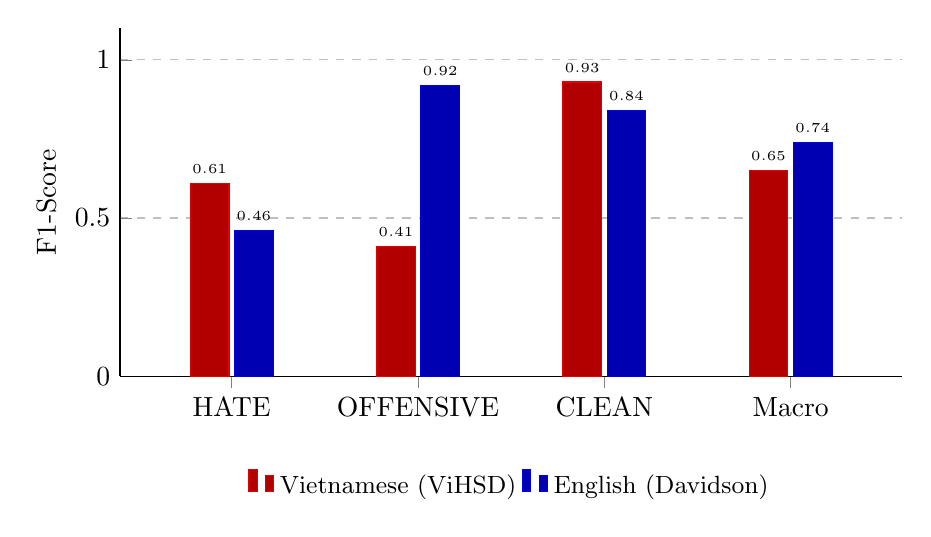
\begin{tikzpicture}
\begin{axis}[
    ybar,
    enlarge x limits=0.2,
    legend style={at={(0.5,-0.25)}, anchor=north, legend columns=-1, draw=none, font=\small},
    ylabel={F1-Score},
    symbolic x coords={HATE, OFFENSIVE, CLEAN, Macro},
    xtick=data,
    nodes near coords,
    nodes near coords align={vertical},
    every node near coord/.append style={font=\tiny\bfseries},
    ymin=0, ymax=1.1,
    width=0.95\textwidth,
    height=6cm,
    bar width=14pt,
    ymajorgrids=true,
    grid style=dashed,
    axis lines*=left,
]
\addplot[fill=red!70!black, draw=red!90!black] coordinates {(HATE,0.61) (OFFENSIVE,0.41) (CLEAN,0.93) (Macro,0.65)};
\addplot[fill=blue!70!black, draw=blue!90!black] coordinates {(HATE,0.46) (OFFENSIVE,0.92) (CLEAN,0.84) (Macro,0.74)};
\legend{Vietnamese (ViHSD), English (Davidson)}
\end{axis}
\end{tikzpicture}

    \caption{F1-score comparison per class and macro-average on the 1,000-sample mixed test set.}
    \label{fig:f1_comp}
\end{minipage}
\vspace{1em}
\begin{minipage}{0.95\textwidth}
    \centering
    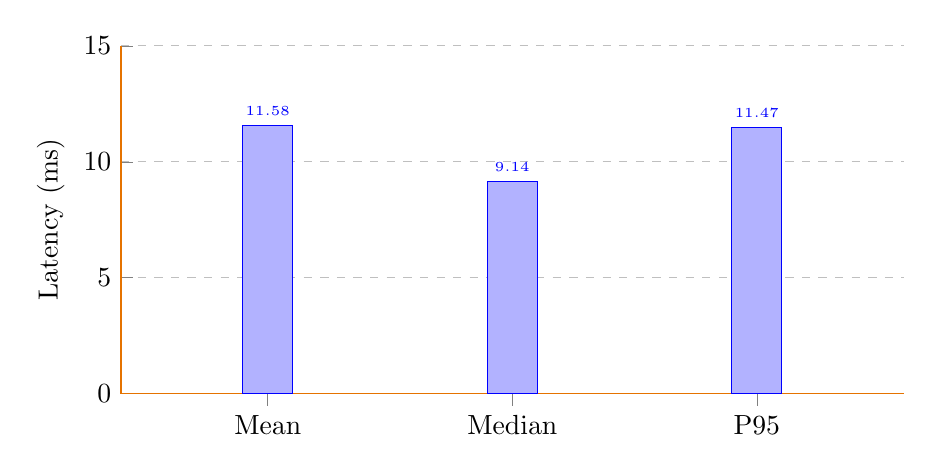
\begin{tikzpicture}
\begin{axis}[
    ybar,
    enlarge x limits=0.3,
    ylabel={Latency (ms)},
    symbolic x coords={Mean, Median, P95},
    xtick=data,
    nodes near coords,
    nodes near coords align={vertical},
    every node near coord/.append style={font=\tiny\bfseries},
    ymin=0, ymax=15,
    width=0.95\textwidth,
    height=6cm,
    bar width=18pt,
    fill=orange!80!black,
    draw=orange!90!black,
    ymajorgrids=true,
    grid style=dashed,
    axis lines*=left,
]
\addplot coordinates {(Mean,11.58) (Median,9.14) (P95,11.47)};
\end{axis}
\end{tikzpicture}

    \caption{End-to-end latency profile (ms) per request.}
    \label{fig:latency_fig}
\end{minipage}
\end{figure}

%!TEX root = main.tex
\section{Analysis}
\label{sec:analysis}

\subsection{Provenance of the 38 Changes (ViHSD)}
\label{sec:provenance}

The aggregate result is neutral; the question is what the 38 changes consist of.
Of the 23 corrections, 16 are \hate{} recoveries (7 from \off{}, 9 from \clean{})
and 7 are \clean{} de-flagging cases (6 from \hate{}, 1 from \off{}).  All 16
\hate{} recoveries have a rule firing with a \hate{} score above the \off{}
score, i.e.\ the rule points in exactly the corrected direction.  The rule
\hate{} score has median 0.7652 (mean 0.7507, range 0.2351--0.9939).

All 7 \clean{} de-flagging cases have a silent rule ($r_H=r_O=0$, so
$\tilde{\mathbf r}=(0,0,1)$).  With $\alpha_H=0.2$ the rule term disappears from
the \hate{} channel and $f_H=0.2\,p_H$, so a comment needs $p_H\ge0.70$ merely
to reach $\tau_H=0.14$; one flagged \hate{} at $p_H\approx0.5$ ends at
$f_H\approx0.10$ and the decision falls back to \clean{}.

The 15 regressions split into 10 rule-driven and 5 threshold-driven cases, and
the split aligns perfectly with direction: all 10 rule-driven cases
(\off{}$\to$\hate{}, \clean{}$\to$\hate{}) have the rule firing in the \hate{}
direction, so fusion trusts lexical \hate{} evidence over the neural label and
the lexicon is wrong about intensity or target.  The \off{} cases are the
expected failure of a phrase lexicon: profanity used as an intensifier rather
than an attack.  The 5 threshold-driven regressions are the mirror image: the
rule is silent, the fused \hate{} score is $0.2\,p_H$, and when $p_H$ falls
below roughly 0.7 the \hate{} channel no longer wins; two miss by exactly
0.001.

\subsection{The Corrections Fusion Does Not Make}
\label{sec:missed_corrections}

Among the 827 AI errors on ViHSD, 148 non-\clean{} comments have the rule
firing in the correct direction and 151 \clean{} comments have the rule
correctly silent, so the rule agrees with the gold label on 299 errors.  Fusion
acts on 23 of them (7.7\%).  The remaining \textbf{132 missed corrections} are
non-\clean{} cases where the rule already points the right way and the hybrid
is still wrong.  Their median rule \hate{} score is 0.7609 (quartiles 0.67--0.85),
indistinguishable from the 0.7652 median of the corrected cases.  They are
missed because the \clean{} channel keeps the full AI weight ($\alpha_C=1.0$),
so a confidently wrong \clean{} cannot be outvoted: the median fused \clean{}
score is 0.97 for missed cases versus 0.46 for corrected ones.

\subsection{What the Rule Channel Responds To (Cue Taxonomy)}
\label{sec:cue_taxonomy}

We annotated the 16 \hate{} recoveries with a multi-label cue taxonomy: ten
contain teencode or abbreviated profanity (\texttt{đ*o}, \texttt{dm},
\texttt{cmnr}), five standard-spelling profanity or an animal slur, and eight
derogatory wording without profanity (\emph{ngu}, \emph{thua}, \emph{nhục}).
The categories overlap.  The channel is therefore not merely a profanity
detector: much of its value comes from derogatory wording a slur list would
miss, and teencode is its largest single category.

\subsection{Component Ablation (Rule Engine Switches)}
\label{sec:ablation}

Re-tuning and re-freezing the fusion once per switch, only one switch matters:
removing the per-entry confidence costs 0.034 standalone macro-F1 (0.5258 to
0.4914), almost all of it on \off{} (F1 0.2389 to 0.0600), and no other
switch moves the standalone engine by more than 0.008.  Rescaling severity
rewrites 1{,}046 of 6{,}680 rule scores yet changes no hybrid decision
($p=1.0$): $\alpha$ and $\tau$ re-tune.  Dropping the obfuscation views trades
recall for precision (firings 1{,}052 $\to$ 779, precision on fired comments
58.75\% $\to$ 69.58\%); fuzzy matching never fires (0 matches), and case-folding
cannot be ablated because all 6{,}680 test comments are already lower-case.
Inside the hybrid no switch leaves noise ($|\Delta|\le0.0012$): the channel
helps as a channel, not through its weights.

\subsection{Language Detection and Routing Quality}
\label{sec:lang_quality}

On the 1000 mixed sample the language detector yields the confusion matrix in
Table~\ref{tab:lang_det}.  Overall per-language accuracy is 93.4\% for each
language.  The 5.6\% (56/1000) fallback to \texttt{multilingual} is the main
source of rule-only degradation (no AI checkpoint for \texttt{mix} or
\texttt{multilingual}).

\begin{table}[H]
\centering
\caption{Language detection confusion matrix (true $\times$ detected) on 1000 mixed samples}
\label{tab:lang_det}
\begin{tabular}{lccccc}
\toprule
True $\backslash$ Detected & en & mix & multilingual & vi & Total \\
\midrule
en                         & 467 & 1   & 30           & 2  & 500 \\
vi                         & 5   & 2   & 26           & 467 & 500 \\
\bottomrule
\end{tabular}
\end{table}

\subsection{Fusion Ablation on Mixed Sample}
\label{sec:ablation_mixed}

Table~\ref{tab:ablation_mixed} compares AI-only, rule-only and fused systems
on the 1000 mixed sample.  On the 941 samples where an AI checkpoint is
available, AI-only (argmax) slightly outperforms fusion at the default
$\alpha=0.70$ (macro-F1 0.8027 vs 0.7937), consistent with the earlier finding
that validation-tuned $\alpha$ converges to $\approx 1.0$ for English and only
the HATE channel keeps a rule contribution ($\alpha_H\approx 0.8$).

\begin{table}[H]
\centering
\caption{Component contributions on the mixed 1000-sample test}
\label{tab:ablation_mixed}
\begin{tabular}{lcccccc}
\toprule
System & $n$ & Accuracy & Macro F1 & HATE F1 & OFFENSIVE F1 & CLEAN F1 \\
\midrule
AI Only (argmax)        & 941  & 0.8884 & \textbf{0.8027} & 0.5750 & 0.9038 & 0.9292 \\
Rule Only (argmax)      & 1000 & 0.6520 & 0.5837 & 0.2963 & 0.7707 & 0.6839 \\
Fused ($\alpha=0.70$)   & 1000 & 0.8700 & 0.7829 & 0.5529 & 0.8824 & 0.9134 \\
Fused ($\alpha=0.70$)   & 941  & 0.8799 & 0.7937 & 0.5660 & 0.8937 & 0.9214 \\
\bottomrule
\end{tabular}
\end{table}
%!TEX root = main.tex
\section{Discussion}
\label{sec:discussion}

\subsection{What the Hybrid Is Good For}
\label{sec:value}

The result is better read as a successful audit: 38 of 6{,}680 decisions change,
each described by a channel, a direction and a mechanism.  Moreover, the
end-to-end bilingual evaluation demonstrates deployment viability (87.10\%
accuracy, 9.07 ms latency, 110.2 texts/s throughput), showing that a hybrid architecture can
be both explainable and production-ready.

\emph{Triage and accountability.}  A queue can sort comments by whether the
decision was rule-supported: a \hate{} decision with a matched span and
$r_H=0.8$ is easier to review than one with no lexical evidence, and the span,
the entry and the arithmetic are what a platform can defend in policy terms.

\emph{Editing and diagnosis.}  Adding a slur variant is a configuration change,
not a retraining run, and an edit affects the \hate{} channel (weight 0.8) far
more than the others.  The decomposition exists only because the channels are
separate: a monolithic classifier improving by 0.0027 macro-F1 would give no
handle on whether the change was lexical or neural.

\subsection{Why Accuracy Does Not Move (Much)}
\label{sec:why_neutral}

First, \emph{coverage is low}: the rule fires on 15.75\% of comments, so a
perfect rule channel could still only change decisions in that subset.  Second,
\emph{the majority class dominates}: with 83\% \clean{}, only the 1{,}132 toxic
comments can improve, and 38 changes is 3.4\% of that support---enough to matter
operationally, too little to move a macro-average beyond its confidence
interval.  Third, \emph{tuning is safety-oriented}: protecting \clean{} and
gating \hate{} on lexical support produces both the de-flagging and the missed
corrections.  Neutrality is a \emph{choice}, not an absence of signal.

\subsection{The Bilingual Asymmetry}
\label{sec:asymmetry_bilingual}

The mixed evaluation reveals a clear language gap: HATE F1 VI 0.6051 vs EN
0.4537 (Vietnamese lexicon has 594 HATE entries versus English 86; Davidson
training only 5.8\% HATE), OFFENSIVE F1 EN 0.9270 vs VI 0.4142 (English
backbone aligns with Davidson's 77.8\% OFFENSIVE majority; ViHSD only 6.65\%
OFFENSIVE), CLEAN F1 VI 0.9344 vs EN 0.8541 (English experiences mild
over-flagging on clean text). This asymmetry is data-driven: lexicon extraction
from corpora with different class priors produces different coverage.

\subsection{Design Implications}
\label{sec:implications_bilingual}

Five changes follow:
\begin{enumerate}
    \item \textbf{Evidence-gated fusion}: when the rule fires strongly against
          a high-confidence \clean{} prediction, abstain or escalate.
    \item \textbf{Separate thresholds per mechanism}: requiring $r_H\ge0.5$
          before the \hate{} channel can override would make the rule-driven
          and threshold-driven paths separately tunable.
    \item \textbf{Per-class calibration} of the \clean{} channel, which currently
          blocks the missed corrections.
    \item \textbf{Balanced English lexicon}: expand HATE entries by merging
          HateXplain/Gab sources and retrain the English rule engine.
    \item \textbf{Multilingual fallback checkpoint}: for \texttt{mix}/\texttt{multilingual}
          samples (5.6\%), route to a multilingual mDeBERTa instead of rule-only.
\end{enumerate}

\subsection{Practical Deployment}
\label{sec:deployment}

The latency profile (9.07 ms mean, 110.2 texts/s throughput) supports synchronous
moderation for text comments.  Routing (5.22 ms) and AI inference (3.85 ms) are the
main components; P95 latency is 12.69 ms.  Tail latency can reach up to 2.1 s during cold-start tokenizer
initialization; this is a one-time cost that can be pre-warmed.  A production
deployment should pre-load both checkpoints and the two rule engines at
startup, cache tokenizer initialization, and set $\alpha$ per language from
validation-frozen weights.
%!TEX root = main.tex
\section{Conclusion}
\label{sec:conclusion}

We presented SensitiveAI, a bilingual language-aware hybrid of lexicon rules
and multilingual transformers for Vietnamese and English hate speech detection.
The system combines a lightweight language detector, language-aware
tokenization, two independently editable rule engines (668 Vietnamese entries,
818 English entries), per-language mDeBERTa-v3-base checkpoints, and
language-aware score fusion with per-class thresholds.

The key results are:
\begin{itemize}
    \item On ViHSD, the hybrid is macro-F1 neutral (0.6575 $\to$ 0.6602,
          $p=0.29$), but its 38 changed decisions are fully decomposable into
          rule-driven and threshold-driven causes, with all 23 corrections
          rule-supported.
    \item On the 9{,}158-sample bilingual evaluation (full ViHSD $+$ Davidson splits), the pipeline
          reaches 87.10\% accuracy, macro-F1 0.7781, 9.07 ms latency and
          110.2 texts/s throughput (serialised run, $\alpha=0.70$, P95 12.69 ms).
    \item The bilingual comparison exposes a structural asymmetry: English
          excels on OFFENSIVE (F1 0.9270) while Vietnamese excels on HATE
          (F1 0.6051); the 818-entry English lexicon still has only 86 HATE
          terms versus 594 for Vietnamese.
    \item Fusion improves calibration: the full-pipeline ECE is 0.076 versus
          0.114 (VI backbone-only) and 0.102 (EN backbone-only), confirming that
          fused scores are better calibrated than raw neural outputs.
\end{itemize}

The broader lesson is methodological: a hybrid evaluated only by its aggregate
metric looks like a null result, whereas the same hybrid decomposed by channel
and direction yields an auditable decision procedure and a design agenda.
Future work includes evidence-gated fusion, balanced English HATE lexicon
expansion, a multilingual fallback checkpoint for code-mixed text, and a
human evaluation of whether the evidence record helps reviewers.
%!TEX root = main.tex
\section{Limitations}
\label{sec:limitations}

\paragraph{Two benchmarks only.}  All results come from ViHSD and Davidson.
The lexicon and cue taxonomy are language-specific; the fusion protocol is
language-agnostic, but it has not been tested on other languages or domains.

\paragraph{One seed per backbone.}  Each backbone was trained once with seed 42,
so neural variance is not estimated and the 0.0027 ViHSD difference is well
inside what seed variance could produce: the tests rule out a large effect, not
a small one.

\paragraph{The Vietnamese rule engine is weaker than designed.}  Validation set
the accent-less alias weight to zero and the negation factor to one, removing
the main defence against dropped diacritics and the discount for negated slurs
visible in the \off{}-as-intensifier regressions.

\paragraph{The English lexicon is imbalanced.}  Expanding from 123 to 818
entries improved OFFENSIVE coverage but left only 86 HATE terms because the
Davidson training split has few HATE documents.  The English HATE F1 (0.46)
remains the weakest class of the bilingual system.

\paragraph{The multilingual fallback is rule-only.}  5.6\% of the mixed sample
falls into \texttt{mix}/\texttt{multilingual}, where no dedicated AI checkpoint
is loaded.  Fusion degenerates to rule-only scoring and depresses macro-F1.

\paragraph{Explanations are not evaluated by humans.}  The evidence record is
faithful for the lexical channel and decomposes the changed decisions, but we
do not measure whether reviewers find it useful, and the cue taxonomy is a
post-hoc annotation.
%!TEX root = main.tex
\section{Ethics}
\label{sec:ethics}

The comments are public ViHSD and Davidson test comments and are masked as
described in Sect.~\ref{sec:data}.  The system is decision support, not
automatic sanctioning: the directional asymmetry, the bilingual gap and the
political false positive show that automatic \hate{} labels from this pipeline
should be reviewed before they affect a user.  The lexicon should be treated as
a governed artefact with a change log, because its entries shape moderation
outcomes.

English and Vietnamese lexicons are not neutral: an entry's charged political
expression can leak into moderation decisions at weight 0.8.  Deployments
should separate \emph{profanity} from \emph{political} entries and weight them
accordingly.  We release no user identifiers and reproduce only corpus text
already public.

\credits
\subsubsection{\discintname}
The authors have no competing interests to declare that are relevant to the
content of this article.

\bibliographystyle{splncs04}
\bibliography{references}

\end{document}
